%卒論概要テンプレート ver. 4.0

\documentclass[uplatex,twocolumn,dvipdfmx]{jsarticle}
\usepackage[top=22mm,bottom=22mm,left=22mm,right=22mm]{geometry}
\setlength{\columnsep}{11mm}
\usepackage[T1]{fontenc}
\usepackage{txfonts}
\usepackage[expert,deluxe]{otf}
\usepackage[dvipdfmx,hiresbb]{graphicx}
\usepackage[dvipdfmx]{hyperref}
\usepackage{pxjahyper}
\usepackage{secdot}





%タイトルと学生番号,名前だけ編集すること
\title{\vspace{-5mm}\fontsize{14pt}{0pt}\selectfont 文書自動添削システムによる学生の文書改善履歴の調査}
\author{\normalsize プロジェクトマネジメントコース 矢吹研究室 1442031   小山隆太郎}
\date{}
\pagestyle{empty}
\begin{document}
\fontsize{10.5pt}{\baselineskip}\selectfont
\maketitle





%以下が本文
\section{序論}
学生が行う研究では,研究だけではなく文書を作成する時間が長い.卒業論文は文量が多く,執筆形式も指摘される.大量の文書を人の目で添削を行うことには限界があり,かかる労力は大きい.

また,文書を自分以外が読んでもわかりやすく書く必要があり,文が長いほど理解が難しくなってしまう場合や,口語が混じり,文書の質が落ちてしまうことがある.

そこで,継続的インテグレーション\cite{a}を用いることで,文書添削を自動化できないか考えた.継続的インテグレーションとは,プログラム全体を常に統合し,動作する状態を指している.

文書自動添削ツールで活用されているRedPenを執筆環境に導入することで,文書の質が向上すると考えた.継続的インテグレーションとRedPenを組み合わせ,文書添削を自動化するツールを構築する.

\section{目的}
RedPenが提供する添削機能は,利用する組織のルールに対応できるように設定が柔軟に行える仕様になっている.
RedPenの文書添削機能を確立し,学生が書く文書の質の向上と,作成時間の短縮を図ることを目的とする.

\section{手法}
本研究の手法について以下に記述する.
\begin{enumerate}
\item 文書自動添削ツールの添削機能を作成する.
\item GitHubにアップロードした文書の添削を自動化する.
\item 作成した添削機能を用いて,文中のミス数の推移を記録する.
\end{enumerate}

\section{結果}
矢吹研究室に所属する3年生が書いた課題研究の概要文の添削を行った際の,エラー数の推移は図\ref{conf}のとおりである.各折れ線が文章1つのミス数の推移を表している.ミス数が減った文書の修正は以下のように行われた.

\begin{enumerate}
\item 「の」,「が」等の接続詞の多用や,同一単語の複数回利用を抑えたことで,文長を短くした.「丁度」,「ちょうど」といった同じ言葉や,数値,アルファベットの表記を統一し,文書を修正した.
\item 「これ」,「あれら」等の指示語の利用を抑えた.「感じる」,「思う」といった感嘆符を使用している文書は,断定系に修正された.
\end{enumerate}

\begin{figure}[htb]
\centering
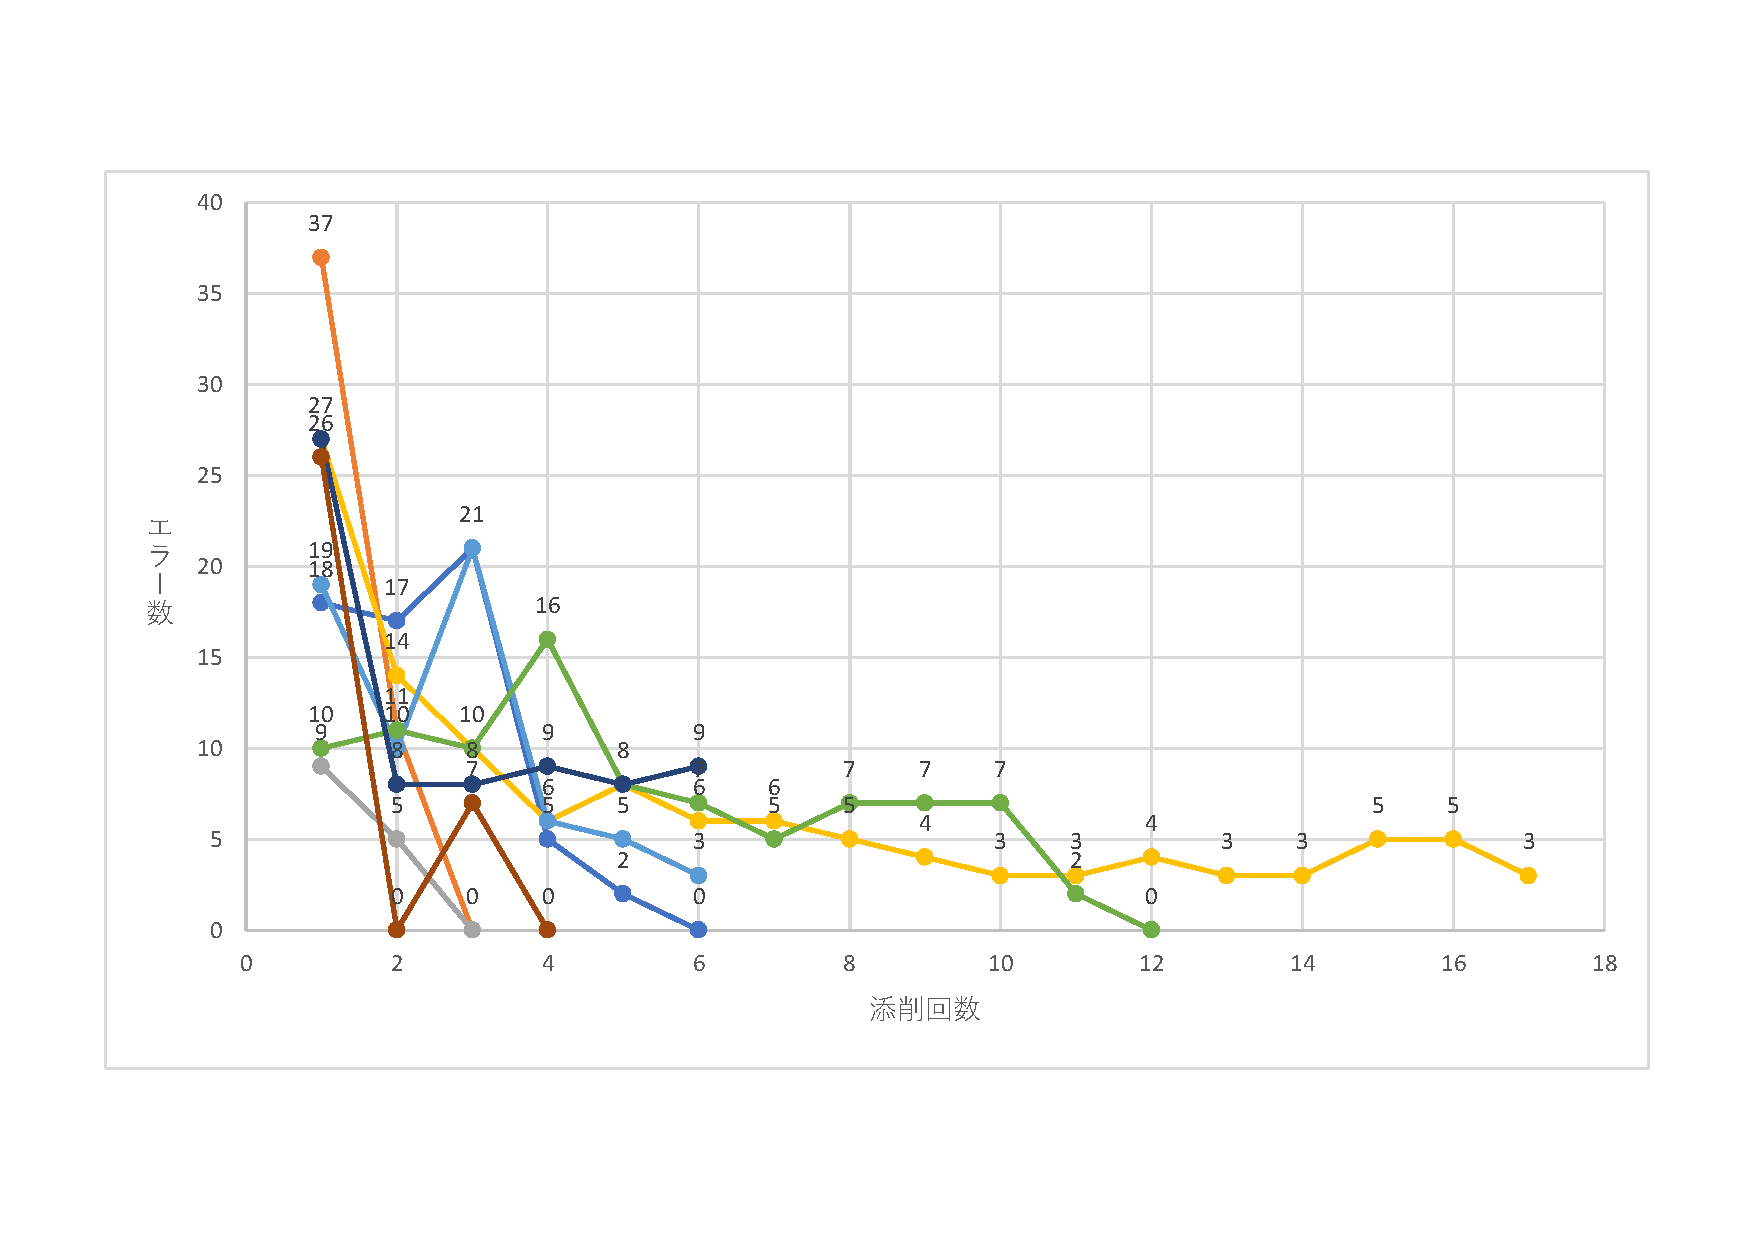
\includegraphics[width=5cm,clip]{redpen.pdf}
\caption{添削ツールを使用した文書の添削項数の推移}\label{conf}
\end{figure}

\section{考察}
文書自動添削ツールの添削機能を作成し,執筆に使用したところ,専門用語を用いて解説する文書を多く見ることができた.「感じる」,「考えられる」等の感嘆符の利用を避け,「考える」と「である調」を使用したことで,研究内容を詳細に解説することに役立った.

\section{結論}
文書添削ツールを使用し,文書添削をしたことで,文中のミスを削減できた.文書添削ツールを利用した際の,文書作成時間が減るか調べたいと考える.




\bibliographystyle{junsrt}
\bibliography{biblio}%「biblio.bib」というファイルが必要.

\end{document}
